% This file was converted to LaTeX by Writer2LaTeX ver. 1.4
% see http://writer2latex.sourceforge.net for more info
\documentclass[a4paper]{article}
\usepackage[ascii]{inputenc}
\usepackage[T1]{fontenc}
\usepackage[english]{babel}
\usepackage{amsmath}
\usepackage{amssymb,amsfonts,textcomp}
\usepackage{color}
\usepackage{array}
\usepackage{supertabular}
\usepackage{hhline}
\usepackage{hyperref}
\hypersetup{pdftex, colorlinks=true, linkcolor=blue, citecolor=blue, filecolor=blue, urlcolor=blue, pdftitle=, pdfauthor=, pdfsubject=, pdfkeywords=}
\usepackage[pdftex]{graphicx}
\makeatletter
\newcommand\arraybslash{\let\\\@arraycr}
\makeatother
% List styles
\newcommand\liststyleWWNumii{%
\renewcommand\labelitemi{${\bullet}$}
\renewcommand\labelitemii{o}
\renewcommand\labelitemiii{${\blacksquare}$}
\renewcommand\labelitemiv{${\bullet}$}
}
\newcommand\liststyleWWNumiii{%
\renewcommand\labelitemi{${\bullet}$}
\renewcommand\labelitemii{o}
\renewcommand\labelitemiii{${\blacksquare}$}
\renewcommand\labelitemiv{${\bullet}$}
}
\newcommand\liststyleWWNumi{%
\renewcommand\theenumi{\arabic{enumi}}
\renewcommand\theenumii{\alph{enumii}}
\renewcommand\theenumiii{\roman{enumiii}}
\renewcommand\theenumiv{\arabic{enumiv}}
\renewcommand\labelenumi{[\theenumi]}
\renewcommand\labelenumii{\theenumii}
\renewcommand\labelenumiii{\theenumiii}
\renewcommand\labelenumiv{\theenumiv}
}
% Page layout (geometry)
\setlength\voffset{-1in}
\setlength\hoffset{-1in}
\setlength\topmargin{1in}
\setlength\oddsidemargin{1in}
\setlength\textheight{7.772499in}
\setlength\textwidth{6.2681in}
\setlength\footskip{0.9602in}
\setlength\headheight{0.5in}
\setlength\headsep{0.4602in}
% Footnote rule
\setlength{\skip\footins}{0.0469in}
\renewcommand\footnoterule{\vspace*{-0.0071in}\setlength\leftskip{0pt}\setlength\rightskip{0pt plus 1fil}\noindent\textcolor{black}{\rule{0.25\columnwidth}{0.0071in}}\vspace*{0.0398in}}
% Pages styles
\makeatletter
\newcommand\ps@Standard{
  \renewcommand\@oddhead{}
  \renewcommand\@evenhead{}
  \renewcommand\@oddfoot{}
  \renewcommand\@evenfoot{}
  \renewcommand\thepage{\arabic{page}}
}
\newcommand\ps@Convertedix{
  \renewcommand\@oddhead{}
  \renewcommand\@evenhead{\@oddhead}
  \renewcommand\@oddfoot{\thepage{}}
  \renewcommand\@evenfoot{\@oddfoot}
  \renewcommand\thepage{\arabic{page}}
}
\newcommand\ps@Convertedviii{
  \renewcommand\@oddhead{}
  \renewcommand\@evenhead{\@oddhead}
  \renewcommand\@oddfoot{\thepage{}}
  \renewcommand\@evenfoot{\@oddfoot}
  \renewcommand\thepage{\arabic{page}}
}
\newcommand\ps@Convertedxiv{
  \renewcommand\@oddhead{}
  \renewcommand\@evenhead{\@oddhead}
  \renewcommand\@oddfoot{\thepage{}}
  \renewcommand\@evenfoot{\@oddfoot}
  \renewcommand\thepage{\arabic{page}}
}
\newcommand\ps@Convertedvii{
  \renewcommand\@oddhead{}
  \renewcommand\@evenhead{\@oddhead}
  \renewcommand\@oddfoot{\thepage{}}
  \renewcommand\@evenfoot{\@oddfoot}
  \renewcommand\thepage{\arabic{page}}
}
\newcommand\ps@Convertedxiii{
  \renewcommand\@oddhead{}
  \renewcommand\@evenhead{\@oddhead}
  \renewcommand\@oddfoot{\thepage{}}
  \renewcommand\@evenfoot{\@oddfoot}
  \renewcommand\thepage{\arabic{page}}
}
\newcommand\ps@Convertedvi{
  \renewcommand\@oddhead{}
  \renewcommand\@evenhead{\@oddhead}
  \renewcommand\@oddfoot{\thepage{}}
  \renewcommand\@evenfoot{\@oddfoot}
  \renewcommand\thepage{\arabic{page}}
}
\newcommand\ps@Convertedxii{
  \renewcommand\@oddhead{}
  \renewcommand\@evenhead{\@oddhead}
  \renewcommand\@oddfoot{\thepage{}}
  \renewcommand\@evenfoot{\@oddfoot}
  \renewcommand\thepage{\arabic{page}}
}
\newcommand\ps@Convertedv{
  \renewcommand\@oddhead{}
  \renewcommand\@evenhead{\@oddhead}
  \renewcommand\@oddfoot{\thepage{}}
  \renewcommand\@evenfoot{\@oddfoot}
  \renewcommand\thepage{\arabic{page}}
}
\newcommand\ps@Convertedxi{
  \renewcommand\@oddhead{}
  \renewcommand\@evenhead{\@oddhead}
  \renewcommand\@oddfoot{\thepage{}}
  \renewcommand\@evenfoot{\@oddfoot}
  \renewcommand\thepage{\arabic{page}}
}
\newcommand\ps@Convertediv{
  \renewcommand\@oddhead{}
  \renewcommand\@evenhead{\@oddhead}
  \renewcommand\@oddfoot{\thepage{}}
  \renewcommand\@evenfoot{\@oddfoot}
  \renewcommand\thepage{\arabic{page}}
}
\newcommand\ps@Convertedx{
  \renewcommand\@oddhead{}
  \renewcommand\@evenhead{\@oddhead}
  \renewcommand\@oddfoot{\thepage{}}
  \renewcommand\@evenfoot{\@oddfoot}
  \renewcommand\thepage{\arabic{page}}
}
\newcommand\ps@Convertediii{
  \renewcommand\@oddhead{}
  \renewcommand\@evenhead{\@oddhead}
  \renewcommand\@oddfoot{\thepage{}}
  \renewcommand\@evenfoot{\@oddfoot}
  \renewcommand\thepage{\arabic{page}}
}
\newcommand\ps@Convertedii{
  \renewcommand\@oddhead{}
  \renewcommand\@evenhead{\@oddhead}
  \renewcommand\@oddfoot{\thepage{}}
  \renewcommand\@evenfoot{\@oddfoot}
  \renewcommand\thepage{\arabic{page}}
}
\newcommand\ps@Convertedi{
  \renewcommand\@oddhead{[Warning: Draw object ignored]}
  \renewcommand\@evenhead{\@oddhead}
  \renewcommand\@oddfoot{\thepage{}}
  \renewcommand\@evenfoot{\@oddfoot}
  \renewcommand\thepage{\arabic{page}}
}
\makeatother
\pagestyle{Standard}
\setlength\tabcolsep{1mm}
\renewcommand\arraystretch{1.3}
\title{}
\author{}
\date{}
\begin{document}
\clearpage\setcounter{page}{1}\pagestyle{Standard}
{\centering  
\includegraphics[width=1.3862in,height=1.0409in]{rahulop-img001.png} \par}
{\centering
\textbf{A PROJECT REPORT }
\par}

{\centering
\textbf{ON}
\par}


\bigskip

{\centering
\textbf{EMOTION BASED AUDIO PLAYER}
\par}


\bigskip

{\centering
\textcolor{black}{SUBMITTED TO THE }
\par}

{\centering
\textcolor{black}{SAVITRIBAI PHULE PUNE UNIVERSITY, PUNE }
\par}


\bigskip

{\centering
\textcolor{black}{IN THE PARTIAL FULFILLMENT OF THE REQUIREMENTS}
\par}

{\centering
\textcolor{black}{FOR THE AWARD OF THE DEGREE OF}
\par}

{\centering
BACHELOR OF ENGINEERING
\par}

{\centering
(ELECTRONICS AND TELECOMMUNICATION) 
\par}


\bigskip

{\centering
SUBMITTED BY
\par}


\bigskip

{\centering
\textbf{RAHUL GAJANAN KATORE}
\par}

{\centering
\textbf{[Exam No. 72159205J]}
\par}

{\centering
UNDER THE GUIDANCE OF
\par}


\bigskip

{\centering
\textbf{MRS. NIKITA CHAVAN}
\par}


\bigskip



\begin{center}

\includegraphics[width=1.1165in,height=1.2in]{rahulop-img002.jpg}
\end{center}

\bigskip


\bigskip

{\centering
\textbf{DEPARTMENT OF ELECTRONICS AND TELECOMMUNICATION}
\par}


\bigskip

{\centering
DR. D.Y. PATIL INSTITUTE OF ENGINEERING, MANAGEMENT \& RESEARCH
\par}

{\centering
\textcolor{black}{AKURDI, PUNE 411044}
\par}


\bigskip


\bigskip

{\centering
\textbf{2023-2024}
\par}

\clearpage\setcounter{page}{2}\pagestyle{Convertedi}

\bigskip

 
\includegraphics[width=1.1181in,height=1.2in]{rahulop-img003.jpg} 


\bigskip

{\centering
\textbf{CERTIFICATE}
\par}


\bigskip

{\centering
\textcolor{black}{This is to certify that the project report entitles}
\par}


\bigskip

{\centering
\textcolor{black}{{}``EMOTION BASED AUDIO PLAYER''}
\par}


\bigskip

{\centering
\textcolor{black}{Submitted by}
\par}

{\centering
\textbf{Rahul Gajanan Katore [Exam No. 72159205J]}
\par}

Is being submitted by Group number: 28 is a record of bonafide work carried out by him/her under the supervision and
guidance of \textbf{Mrs. Nikita Chavan} in partial fulfillment of the requirement for
\textbf{\textcolor{black}{Bachelor of Engineering}} (\textcolor{black}{(E\&TC Engineering}) -- 2019 course of
Savitribai Phule Pune University, Pune in the academic year \textbf{2023-2024.}


\bigskip


\bigskip


\bigskip


\bigskip


\bigskip

\begin{flushleft}
\tablefirsthead{}
\tablehead{}
\tabletail{}
\tablelasttail{}
\begin{supertabular}{m{2.4233599in}m{1.9823599in}m{1.96436in}}
\textbf{\textcolor{black}{\ \ \ Mrs. Nikita Chavan}} &
\centering \textbf{\textcolor{black}{\ Mrs. D. N. Hire}} &
\centering\arraybslash \textbf{\textcolor{black}{Dr. Priya Charles}}\\
\centering \textcolor{black}{Guide} &
\centering \textcolor{black}{\ \ \ \ \ \ \ Project coordinators} &
\centering\arraybslash \textcolor{black}{Head}\\
{\centering \textcolor{black}{Department of E\&TC}\par}

\centering \textcolor{black}{Engineering} &
\centering \textcolor{black}{Department of E\&TC Engineering} &
\centering\arraybslash \textcolor{black}{\ Department of E\&TC Engineering}\\
\end{supertabular}
\end{flushleft}

\bigskip


\bigskip


\bigskip

{\centering
\textbf{Dr. Anupama V. Patil}
\par}

{\centering
\textcolor{black}{Principal,}
\par}

{\centering
\textcolor{black}{Dr. D.Y. Patil Institute of Engineering, Management \& Research Akurdi Pune }
\par}


\bigskip


\bigskip

\textcolor{black}{Place: Pune}

\textcolor{black}{Date:}

\clearpage\setcounter{page}{1}\pagestyle{Convertedii}
{\centering
\textbf{DECLARATION}
\par}


\bigskip

\textcolor{black}{We hereby declare that the entire project work entitled ``EMOTION BASED AUDIO PLAYER'' is a project
report of original work done by us and to the best of my knowledge and belief. No part of it has been submitted for any
degree or diploma of any Institution previously. This Project work is submitted to Savitribai Phule Pune University,
Pune in the Dr. D.Y. Patil Institute of Engineering, Management and Research, Akurdi, Pune during the academic year
2022-2023.}


\bigskip


\bigskip


\bigskip

\textcolor{black}{Place:\ \ Signature of Students}

\textcolor{black}{Date:\ \ 1. Rahul Katore}


\bigskip


\bigskip


\bigskip

{\centering
\textbf{ACKNOWLEDGEMENT}
\par}


\bigskip

\textcolor{black}{We express our sincere gratitude towards the faculty members who made this project work successful.}

\textcolor{black}{We would like to express our thanks to our guide }\textbf{\textcolor{black}{Mrs. Nikita Chavan
}}\textcolor{black}{for his/her wholehearted co-operation and valuable suggestions, technical guidance throughout the
project work.}

\textcolor{black}{Special thanks to our H.O.D. }\textbf{\textcolor{black}{Dr. Priya Charles}}\textcolor{black}{ for her
kind official support and encouragement. We are also thankful to our project coordinators
}\textbf{\textcolor{black}{Mrs. D. N. Hire}}\textcolor{black}{ for their valuable guidance.}

\textcolor{black}{Finally, we would like to thank all our staff members in the E\&TC Department who helped us directly
or indirectly to complete this work successfully.}


\bigskip


\bigskip

Rahul Katore 72159205J

\textcolor{black}{(BE E\&TC Engineering)}


\bigskip


\bigskip

\clearpage\clearpage\setcounter{page}{1}\pagestyle{Convertediii}

\bigskip

{\centering
\textbf{\textcolor{black}{ABSTRACT}}
\par}


\bigskip

Current research has confirmed that individuals respond significantly to music, with a profound impact on their
cognitive activity. The average Indian dedicates up to four hours daily to listening to songs, often choosing music
based on their mood and interests. This project focuses on developing an application to recommend songs to users based
on their mood, leveraging facial expressions as a form of nonverbal communication.

Computer vision, an interdisciplinary field, facilitates a high-level understanding of digital images or videos by
computer systems. In this application, computer vision components are employed to discern the user's emotion through
facial expressions. Once the emotion is identified, the system suggests a playlist tailored to that emotion, saving
users considerable time compared to manual song selection.

The emotion-based music player also keeps track of user details, including the play count for each song, categorizes
songs based on genre and interest level, and dynamically reorganizes the playlist. Furthermore, the system notifies
users about songs that have never been played, allowing for potential deletion or modification.

This holistic approach aims to enhance the user experience by providing personalized music recommendations while
efficiently managing and organizing their music preferences based on facial expressions and usage patterns


\bigskip


\bigskip

\clearpage\setcounter{page}{1}\pagestyle{Convertediv}
{\centering
\textbf{\textcolor{black}{Contents}}
\par}


\bigskip

\textcolor{black}{CERTIFICATE{\dots}{\dots}{\dots}{\dots}{\dots}{\dots}{\dots}{\dots}{\dots}{\dots}{\dots}{\dots}{\dots}{\dots}{\dots}{\dots}{\dots}{\dots}{\dots}{\dots}{\dots}{\dots}{\dots}{\dots}{\dots}{\dots}{\dots}{\dots}{\dots}{\dots}{\dots}{\dots}{\dots}{\dots}2}

\textcolor{black}{DECLARATION{\dots}{\dots}{\dots}{\dots}{\dots}{\dots}{\dots}{\dots}{\dots}{\dots}{\dots}{\dots}{\dots}{\dots}{\dots}{\dots}{\dots}{\dots}{\dots}{\dots}{\dots}{\dots}{\dots}{\dots}{\dots}{\dots}{\dots}{\dots}{\dots}{\dots}{\dots}{\dots}{\dots}.3}

ACKNOWLEDGEMENT{\dots}{\dots}{\dots}{\dots}{\dots}{\dots}{\dots}{\dots}{\dots}{\dots}{\dots}{\dots}{\dots}{\dots}{\dots}{\dots}{\dots}{\dots}{\dots}{\dots}{\dots}{\dots}{\dots}{\dots}{\dots}{\dots}{\dots}{\dots}{\dots}...3

\textcolor{black}{ABSTRACT{\dots}{\dots}{\dots}{\dots}{\dots}{\dots}{\dots}{\dots}{\dots}{\dots}{\dots}{\dots}{\dots}{\dots}{\dots}{\dots}{\dots}{\dots}{\dots}{\dots}{\dots}{\dots}{\dots}{\dots}{\dots}{\dots}{\dots}{\dots}{\dots}{\dots}{\dots}{\dots}{\dots}{\dots}.{\dots}4
}

\setcounter{tocdepth}{10}
\renewcommand\contentsname{}
\tableofcontents
\clearpage\setcounter{page}{1}\pagestyle{Convertedv}
{\centering
\textbf{LIST OF FIGURES}
\par}

\setcounter{tocdepth}{10}
\renewcommand\contentsname{}
\tableofcontents

\bigskip

\setcounter{tocdepth}{10}
\renewcommand\contentsname{}
\tableofcontents

\bigskip

\setcounter{tocdepth}{10}
\renewcommand\contentsname{}
\tableofcontents

\bigskip

\setcounter{tocdepth}{10}
\renewcommand\contentsname{}
\tableofcontents

\bigskip


\bigskip


\bigskip


\bigskip


\bigskip


\bigskip


\bigskip


\bigskip


\bigskip

{\centering
\textbf{LIST OF TABLES}
\par}

\setcounter{tocdepth}{10}
\renewcommand\contentsname{}
\tableofcontents

\bigskip


\bigskip


\bigskip


\bigskip


\bigskip


\bigskip


\bigskip


\bigskip


\bigskip

\clearpage\setcounter{page}{1}\pagestyle{Convertedvi}
{\bfseries
\hypertarget{gjdgxs}{}CHAPTER 1 INTRODUCTION}

{\bfseries
\hypertarget{30j0zll}{}1.1 INTODUCTION}

Emotions encompass the physical sensations linked to one's mood, temperament, character, or individuality. Paul Ekman,
in 1972, classified basic emotions as anger, disgust, fear, happiness, sadness, and surprise.

Facial expressions manifest through movements, actions, or positions of facial muscles, conveying an individual's
emotional state. While facial expressions can be voluntary, with a person controlling facial features to convey a
specific emotion, they are primarily involuntary, tightly linked to genuine emotions. For example, an individual might
furrow their eyebrows and frown to express irritation or intentionally relax facial muscles to appear unaffected.

Despite efforts to conceal current emotions, facial expressions often reveal them involuntarily, typically within the
first few microseconds before returning to a neutral expression. Since Darwin's work in 1872, behavioral scientists
have actively researched and analyzed facial expression detection, making significant progress in developing computer
systems for understanding and interpreting individuals' facial expressions in communication.

The {\textquotedbl}Emotion-based Music Player{\textquotedbl} is a tool designed to detect an individual's emotion and
play a curated list of tunes accordingly. Initially, the person expresses their emotion through facial expression,
which the device then detects, analyzes, and interprets. Subsequently, the music player selects songs that align with
the detected emotion. The focus of the system is on analyzing facial expressions without considering head or face
movements

{\bfseries
\hypertarget{1fob9te}{}1.2 GOALS \& OBJECTIVES / SCOPE}

\liststyleWWNumii
\begin{itemize}
\item \textcolor{black}{The emotion-based music player is a valuable application tailored for music enthusiasts
possessing a smartphone and internet connectivity. This user-friendly software is accessible to anyone who establishes
a profile on the platform. The application is strategically crafted to meet the following user requirements:}
\item \textcolor{black}{Account Creation or Registration, Sign-Up, and Sign-In for System Reliability}
\item \textcolor{black}{Song Management: Addition, Deletion, and Updates}
\item \textcolor{black}{Personalized Playlist Creation}
\item \textcolor{black}{Music Recommendations}
\item \textcolor{black}{Emotion Capture through Camera Functionality}
\item \textcolor{black}{Users can seamlessly navigate and engage with the application, ensuring a tailored and enjoyable
music listening experience.}
\end{itemize}
{\bfseries
\hypertarget{3znysh7}{}1.3 MOTIVATION}

As an avid music enthusiast, I have consistently believed that music players should offer more than just playing songs
and allowing users to curate playlists. A music player should exhibit intelligence and adapt to the user's preferences,
aiding in the seamless organization and automated playback of songs without requiring extensive user effort. The
Emotion-based music player establishes an enhanced platform for all music enthusiasts, ensuring the automated selection
and regular updating of playlists. This feature empowers users to effortlessly organize and play songs in accordance
with their moods. Moreover, the player provides on-the-go suggestions for users to modify songs, utilizing the EMO
algorithm to calculate song weight, thereby facilitating a more personalized and well-organized playlist experience.


\bigskip

{\bfseries
\hypertarget{2et92p0}{}1.4 PROBLEM STATEMENT }

The impact of music on an individual's emotions is widely acknowledged. Whether for primitive or modern man, after a day
of toil and hard work, the soothing melody of music provides a means to relax and unwind. Research even supports the
notion that the rhythm itself acts as a powerful tranquilizer.

However, the challenge for many lies in the selection of music, particularly finding songs that align with one's current
emotional state. Confronted with lengthy, unorganized music lists, individuals often feel demotivated to sift through
and locate specific songs. Consequently, they may resort to randomly choosing songs within the music folder, leading to
a mismatch with their current emotions. For instance, someone feeling sad might prefer heavy rock music to channel
their emotions, but the arduous task of manually searching through a vast playlist proves impractical. As a result,
individuals often opt to play songs randomly or select the {\textquotedbl}play all{\textquotedbl} option for their
entire collection.

This conventional approach to searching and selecting songs has been in practice for several years, causing people to
grow weary of its limitations. The need for a more efficient and personalized method of music selection has become
increasingly apparent over time.

\clearpage\setcounter{page}{1}\pagestyle{Convertedvii}
{\bfseries
\hypertarget{tyjcwt}{}CHAPTER 2 LITERATURE SURVEY }

A literature survey is gathering information on previous work done related to your project. It contains the research
study year, researchers name, technologies used and drawbacks of the system. 


\bigskip

{\bfseries
\hypertarget{3dy6vkm}{}2.1 LITERATURE SERVEY }

{\centering
\hypertarget{1t3h5sf}{}\textbf{\textit{\textcolor{black}{Table 2. 1 Overview of literature survey}}}
\par}

\begin{flushleft}
\tablefirsthead{}
\tablehead{}
\tabletail{}
\tablelasttail{}
\begin{supertabular}{|m{0.5358598in}|m{2.1559598in}|m{1.6115599in}|m{2.1143599in}|}
\hline
\centering \textbf{Sr. No.} &
\centering \textbf{Topic} &
\centering \textbf{Author and Year} &
\centering\arraybslash \textbf{Summary/Details}\\\hline
~

~

01  &
Music stands as one of the most universally embraced cultures and languages, transcending boundaries and appealing to
people of all backgrounds and types. &
~

Barbara Raskauskas, 

Oct 2009  &
~

Music provides enjoyment and communicates with us, irrespective of whether it contains lyrics or not.\\\hline
~

~

02  &
~

Individuals are drawn to music for similar reasons that attract them to substances, gambling, and delectable food, as
indicated by recent research. &
~

Emily Sohn, Sept-

Oct 2011  &
The research demonstrated that when individuals listen to harmonious or melodic elements that resonate with them, the
human brain releases dopamine, a chemical associated with addiction and motivation.

~
\\\hline
~

03  &
~

\textcolor[rgb]{0.05882353,0.05882353,0.05882353}{Detecting facial expressions in an individual can be achieved by
comparing them with similar expressions.}.  &
~

Mary Duenwald, 

Mar 2005  &
Scientists have conducted numerous studies and research, revealing that facial expressions globally tend to fall roughly
into seven categories.\\\hline
\end{supertabular}
\end{flushleft}

\bigskip

{\bfseries
\hypertarget{4d34og8}{}2.2 DESCRIPTION }

In 2009, Barbara Raskauskas published an article asserting that music serves as a universally accepted culture and
language, embraced by people of all kinds. Raskauskas emphasized the ability of music to fill silence, convey cultural
upbringing, and provide pleasure, asserting its universality as a source of enjoyment even for individuals with hearing
impairments. She stated that finding joy in music is a universal experience.

According to Emily Sohn in 2011, people's love for music shares similarities with their attraction to drugs, gambling,
and delectable food, as indicated by recent research. Sohn highlighted the study's findings, demonstrating that
listening to harmonious or melodic elements induces the release of dopamine in the human brain, contributing to
feelings of addiction and motivation.

Detecting facial expressions in individuals involves comparing them with similar expressions, as highlighted in a 2005
article by Mary Duenwald. Duenwald summarized various studies revealing that facial expressions worldwide can be
broadly categorized into seven distinct categories.\textbf{ }

\clearpage\setcounter{page}{1}\pagestyle{Convertedviii}
{\bfseries
\hypertarget{2s8eyo1}{}CHAPTER 3 PROPOSED SOLUTION }

The device architecture of the Emotion-based music player is illustrated in Figure 3.1. The application is constructed
employing the architectural model-view-controller pattern, a widely utilized framework in architecture. In this
context, the application is divided into three primary logical components: the model, the view, and the controller


\bigskip

{\bfseries
\hypertarget{17dp8vu}{}3.1 INTRODUCTION\ \ }

{\centering  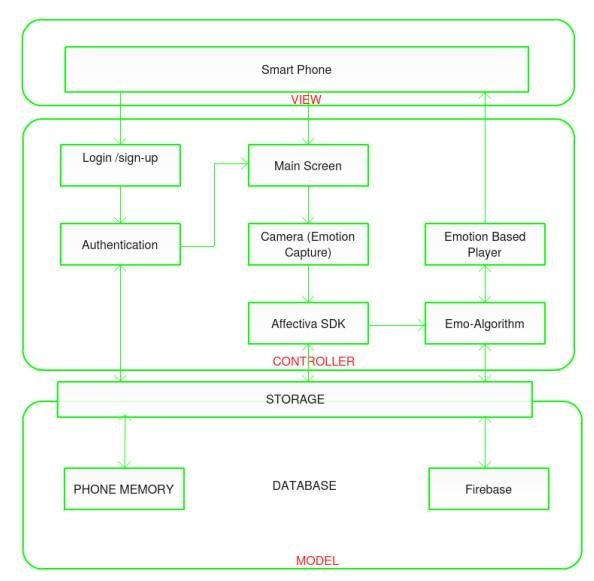
\includegraphics[width=4.3811in,height=3.3437in]{rahulop-img004.jpg} \par}
{\centering
\hypertarget{3rdcrjn}{}\textbf{\textcolor{black}{Figure 3. 1 System Architecture of Emotion-Based Music Player}}
\par}


\bigskip

View: The topmost layer is where the end-user engages with the software by clicking buttons, entering details, accessing
the camera, selecting a radio button, uploading songs, etc. This layer is responsible for displaying all information or
a portion of data to the user based on the application's requirements. Additionally, it acts as a bridge facilitating
communication between the user and the application.

Controller: Positioned in the middle layer of the application, the controller houses the business logic and core
functionality. When the user interacts with the application, this layer processes the response. From login procedures
to displaying playlists, all background functions belong to this layer. It encompasses functions and the EMO algorithm
crucial for song segregation and sending output to the view layer.

Model: This component is responsible for maintaining user data. The Emotion-based music player utilizes Google Firebase
for storing user data, providing a useful repository for user profiles and preferences. The application also stores
certain temporary data on the device.

{\bfseries
\hypertarget{26in1rg}{}3.2 SYSTEM OVERVIEW}

This section delineates the design and functional aspects of the application. The Emotion-Based music player is
installed on a mobile device, allowing users to access their customized playlists and play songs based on their
emotions. Figure 3.2 provides an overview of the application.

 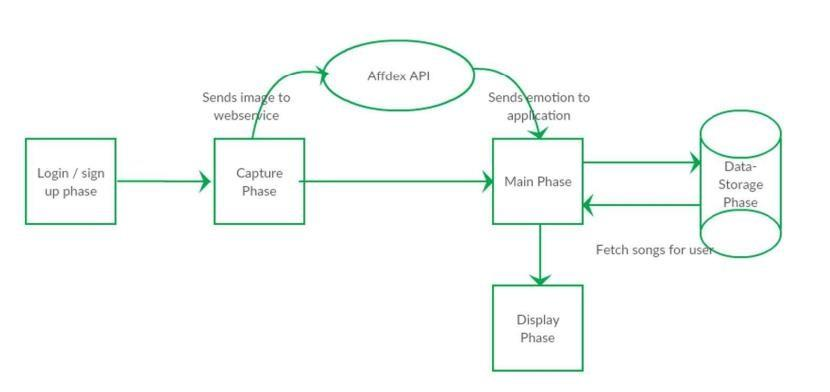
\includegraphics[width=6.2681in,height=2.7453in]{rahulop-img005.jpg} 

{\centering
\hypertarget{lnxbz9}{}\textbf{\textit{\textcolor{black}{Figure 3. 2 System Flow of Emotion-Based Music Player}}}
\par}

Login/Sign-Up Phase: Users are required to create a profile to store personal data. If the user already has an account,
they can log in to access personalized playlists and songs. Upon login, the user's profile is saved until manual
logout. User-added songs and their details, such as category and interest level, are recorded by the system.

Emotion Capture Phase: After authentication, the application seeks the user's permission to access media and photos,
capturing the user's image via the camera.

Affdex API: The captured image is sent to the Affdex SDK for processing. The SDK analyzes the image, and the image
comments are relayed back to the application.

Emo-Phase: In this stage, the application receives image data and identifies the emotion based on a predefined
threshold. This emotion is then sent to the database to retrieve the emotion-based playlist.

Display Phase: Songs are organized using the EMO algorithm, and the user can play any song from the displayed list.
Users can add, remove, and modify songs, as well as adjust the category and interest level at any time. The application
includes a recommendation tab, notifying users of seldom-played songs.


\bigskip

\clearpage{\bfseries
\hypertarget{35nkun2}{}3.3 SYSTEM REQUIREMENTS}

The minimum requirements for developing this application are as follows:


\bigskip

\textbf{Hardware Requirements:}

Processor: 2 GHz

RAM: 1 GB

Browser Compatibility:


\bigskip

Chrome 51 or higher

Firefox 47 or higher

Opera 37

Edge 10586

Database:


\bigskip

Firebase

NoSQL

API:


\bigskip

Affective Emotion Recognition API 

\clearpage\setcounter{page}{1}\pagestyle{Convertedix}
{\bfseries
\hypertarget{1ksv4uv}{}CHAPTER 4 PROPOSED METHODOLOGY}

This chapter introduce us regarding the example model (GUI) within which it renowned us however project seem like and
implementation detail of first module. 

{\bfseries
\hypertarget{44sinio}{}4.1 PROPOSED MODEL}

 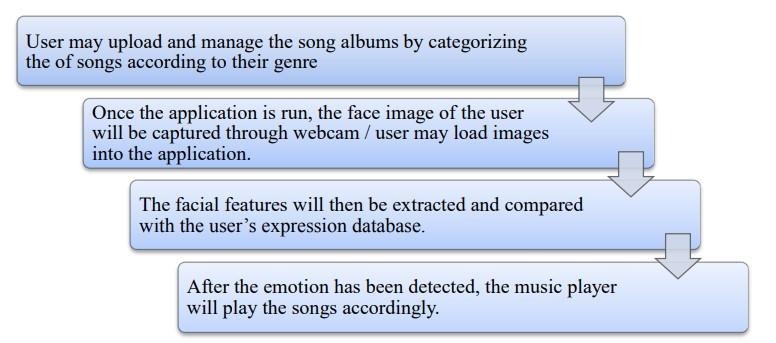
\includegraphics[width=6.2681in,height=2.6252in]{rahulop-img006.jpg} 

{\centering
\hypertarget{2jxsxqh}{}\textbf{\textit{\textcolor{black}{Figure 4. 1Working of The Proposed Model}}}
\par}


\bigskip

From the developer side, as for this FYP, the proposed version may be focusing on two primary capabilities, first is
expression detection and second the list of songs played for each class of emotion. As for expression detection, the
machine is designed specially to hit upon the 4 main expressions, which might be happy, unhappy, normal and surprised.
Alternatively, there might be songs ready available in every category. After the emotion of the person is detected, the
machine will play ten songs through the music player. 

\ Except, there can be units of nevertheless photos with the four special expressions available in the database of
facial features detection. It will likely be used for contrast functions. After the photo of the person is loaded, the
capabilities (lip and eyes) of the user may be extracted by using the system. The gadget will then analyze the
situation of the functions and do a comparison with the units of emotions inside the database. The system will discover
processed photographs for instance as happy whilst the situation of the features is nearest to the ``satisfied
emotion'' within the database. 

\ As for the consumer facet, the user might be capable of personalizing the songs in every category in line with their
taste. Some might choose sentimental music when she is unhappy however some may choose a few countryside tunes. There
can be no restriction on songs to be kept in each category. The consumer will ought to launch the system for you to
start the proposed model. Once the device is started, the person can select to either pick songs or to directly
technique the modern emotion. A list of songs can be performed routinely after the gadget is achieved with the
translation. Users can pick to alternate the modern-day emotion after the listing of a song is being played by using
repeating the image loading or capturing technique. 


\bigskip

{\bfseries
\hypertarget{z337ya}{}4.2 ALGORITHM }


\bigskip

\textbf{EMO-algorithm}


\bigskip

\textbf{Data:} Interest level and category while adding a song, count of song, a user changing song category, skipping
the song 

\ \textbf{Result:} Customize music list based on emotion-recognized initialization; 

\begin{center}
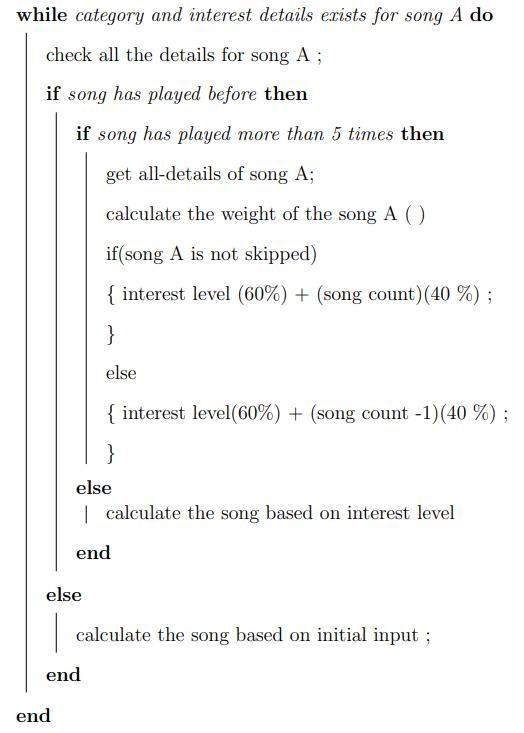
\includegraphics[width=3.7709in,height=5.2083in]{rahulop-img007.jpg}
\end{center}

\bigskip

{\centering [Warning: Draw object ignored]\par}

\bigskip

In this stage, the EMO algorithm determines the categorization of songs. When a user adds a song to the application, the
system collects details such as the song category and user interest level. Upon the user's interaction with the
application, the EMO algorithm takes various factors into account to customize the playlist. The factors influencing
the calculation of the song weight include:

Category and interest level

Number of times the song has been played

If a song has never been played

If a song has been played less than 5 times

If a song has been played more than 5 times

Number of times the song has been skipped

The EMO algorithm employs the following formula to calculate the song weight, emphasizing the song's interest level and
the frequency of play:

Song Weight

=

(

60

\%

)

{\texttimes}

number of times played

+

(

40

\%

)

{\texttimes}

song interest level

Song Weight=(60\%){\texttimes}number of times played+(40\%){\texttimes}song interest level


\bigskip

This algorithm accommodates instances where the user skips a song, presuming a lack of interest and subsequently
reducing the song's weight.

Utilizing Algorithm 1, the application classifies songs based on each emotion, presenting them to the user. Each user
benefits from a personalized playlist, allowing the addition of new songs to the music player. Through the EMO
algorithm, all songs are dynamically reorganized at runtime, recalculating song weights whenever the user interacts
with the application.\textbf{ }

\clearpage\setcounter{page}{1}\pagestyle{Convertedx}
{\bfseries
\hypertarget{3j2qqm3}{}CHAPTER 5 SYSTEM RCHITECTURE}

This chapter introduces us to the prototype model (GUI) which it has known us what the project looks like and the
implementation detail of the first module. 

{\centering  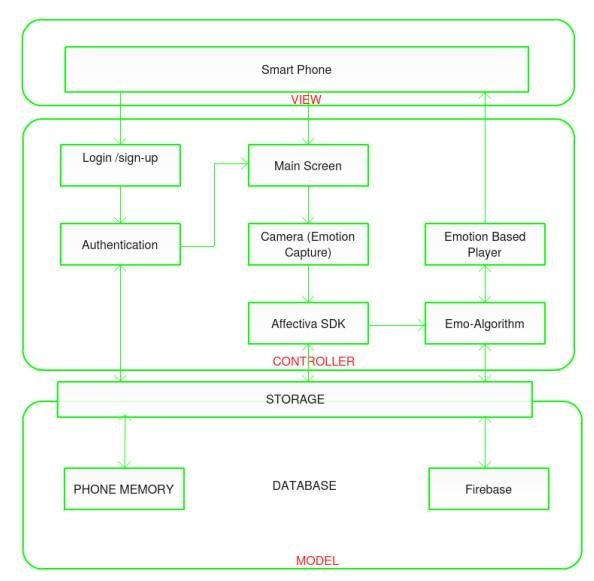
\includegraphics[width=4.448in,height=3.1665in]{rahulop-img004.jpg} \par}
\hypertarget{1y810tw}{}\textbf{Figure 5. 1 The prototype model of the system shows the activity of creating of
prototypes of applications, that is, incomplete versions of the product being developed. }


\bigskip


\bigskip

\clearpage\setcounter{page}{1}\pagestyle{Convertedxi}
{\bfseries
\hypertarget{4i7ojhp}{}CHAPTER 6 DESIGN}

{\bfseries
\hypertarget{2xcytpi}{}6.1 As-Is-System}

[Warning: Draw object ignored]

\begin{center}
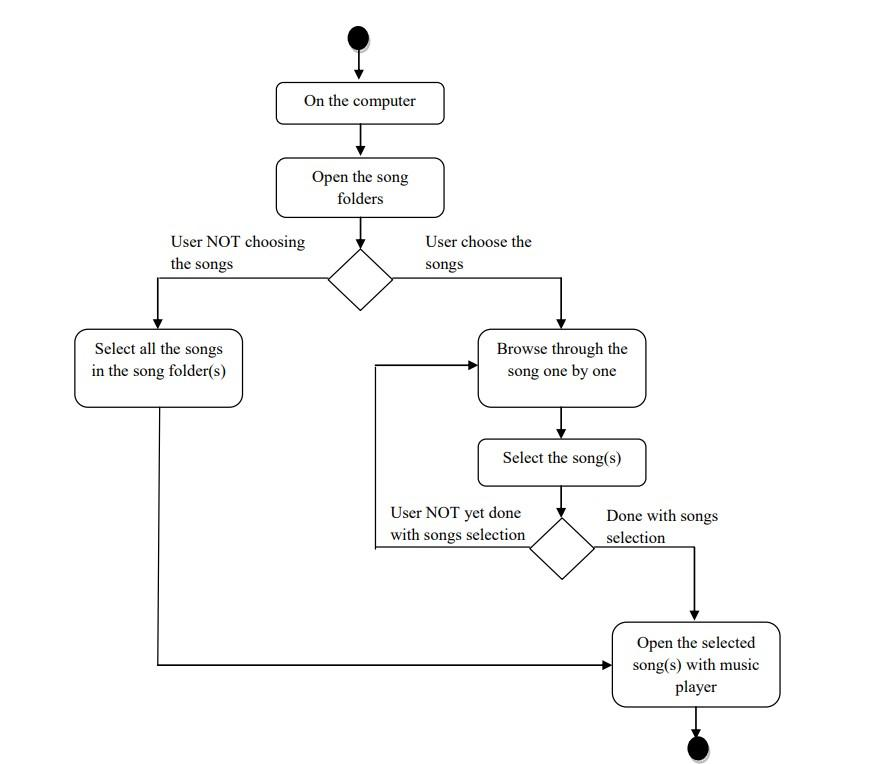
\includegraphics[width=5.7917in,height=5.6563in]{rahulop-img008.jpg}
\end{center}

\bigskip


\bigskip


\bigskip


\bigskip


\bigskip


\bigskip


\bigskip


\bigskip


\bigskip


\bigskip


\bigskip


\bigskip


\bigskip


\bigskip


\bigskip


\bigskip


\bigskip


\bigskip


\bigskip


\bigskip


\bigskip


\bigskip


\bigskip


\bigskip


\bigskip


\bigskip


\bigskip


\bigskip


\bigskip


\bigskip


\bigskip


\bigskip


\bigskip


\bigskip


\bigskip

\clearpage{\bfseries
\hypertarget{1ci93xb}{}6.2 To-Be-System}

 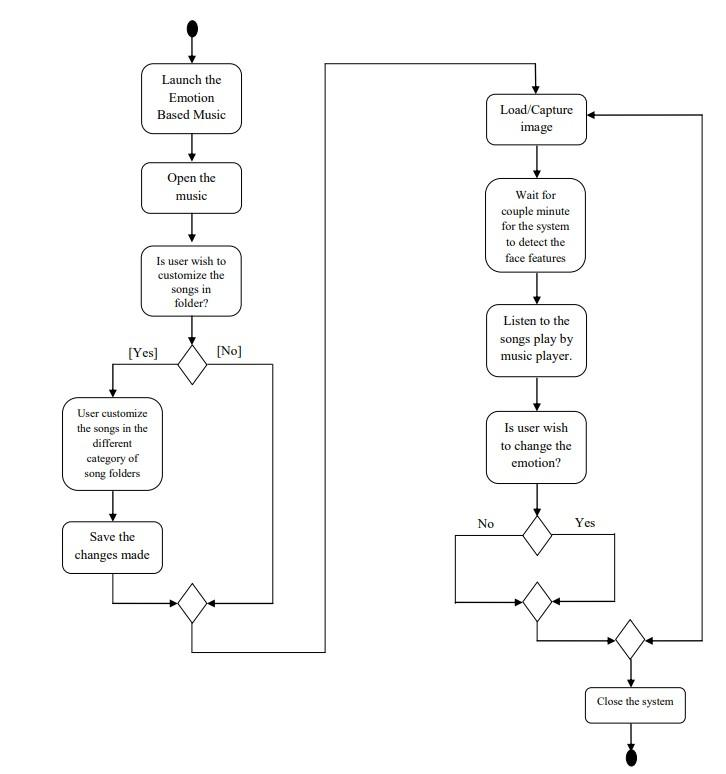
\includegraphics[width=5.4327in,height=5.0307in]{rahulop-img009.jpg} 

{\centering
\hypertarget{3whwml4}{}\textbf{\textcolor[rgb]{0.26666668,0.32941177,0.41568628}{Figure 6. 2 The To-Be user process
flowchart}}
\par}


\bigskip


\bigskip


\bigskip

{\bfseries
\hypertarget{2bn6wsx}{}6.3 UML DIAGRAM}


\bigskip

The Unified Modeling Language (UML) is a versatile modeling language within the realm of software engineering, devised
to establish a standardized method for visualizing system designs. UML serves as a means to depict a system's
architectural plans through diagrams, encompassing elements such as:

Various activities or tasks.

Individual components constituting the system.

Interactions between different software components.

System execution details.

Entity interactions.

External user interface.

{\bfseries
\hypertarget{qsh70q}{}6.3.1 CLASS DIAGRAM}

[Warning: Draw object ignored]Class diagrams stand out as the most prevalent diagrams employed in UML. Comprising
classes, interfaces, associations, and collaborations, a class diagram essentially portrays the object-oriented
perspective of a system, emphasizing its static characteristics.

\begin{center}
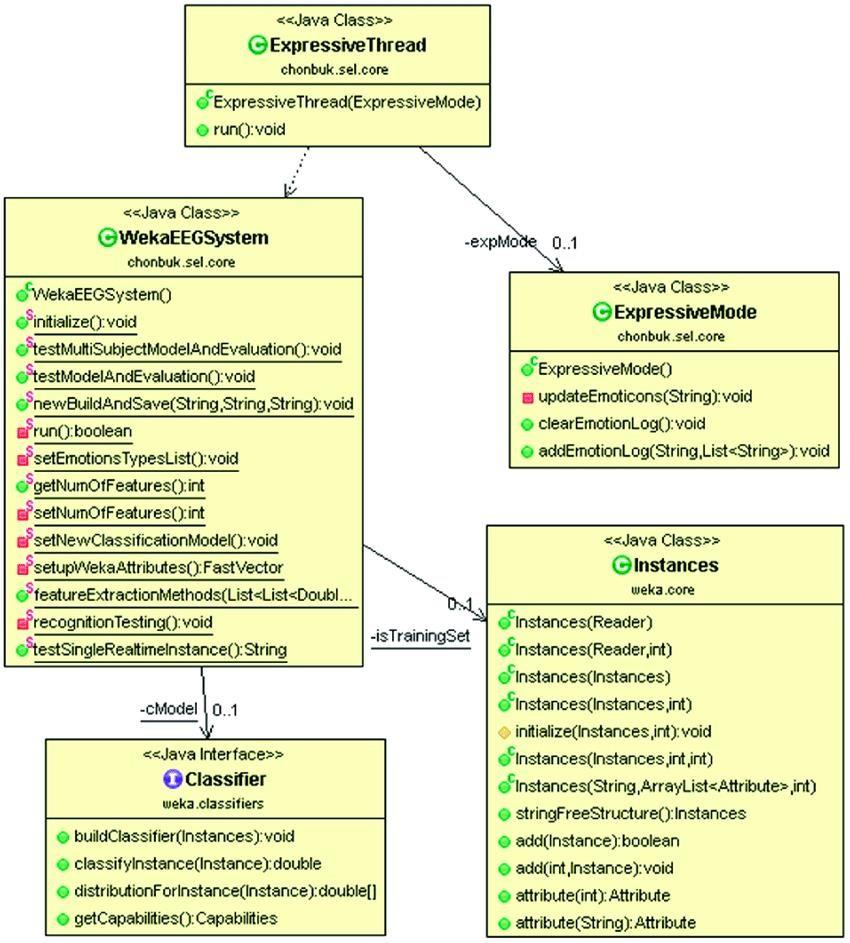
\includegraphics[width=6.4374in,height=6.4272in]{rahulop-img010.jpg}
\end{center}

\bigskip

\clearpage{\bfseries
\hypertarget{3as4poj}{}6.3.2 SEQUENCE DIAGRAM}


\bigskip

A sequence diagram in the Unified Modeling Language (UML) is a specific type of interaction diagram that illustrates how
processes collaborate and the sequence in which they operate. It is structured akin to a Message Sequence Chart. This
diagram places emphasis on the chronological order of messages, portraying objects along the X-axis and depicting the
order of messages on the Y-axis in increasing time. The line representing an object's existence is termed the object
lifeline.

User object has any PC related problem occurs then the user able to register this type of problem. 

User is responsible for creating all other objects. 

 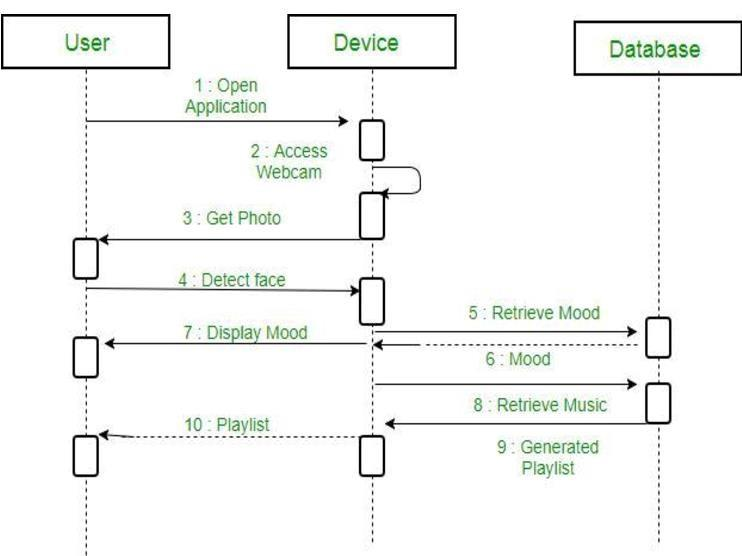
\includegraphics[width=6.2311in,height=4.6701in]{rahulop-img011.jpg} 

{\centering
\hypertarget{1pxezwc}{}\textbf{\textcolor{black}{Figure 6. 4 Sequence Diagram}}
\par}

\clearpage\setcounter{page}{1}\pagestyle{Convertedxii}
{\bfseries
\hypertarget{49x2ik5}{}CHAPTER 7 FUTURE SCOPE \ }


\bigskip

{\bfseries
\hypertarget{2p2csry}{}7.1 FUTURE SCOPE}


\bigskip

The software can be stepped forward by using enhancement and functionality. 

\liststyleWWNumiii
\begin{itemize}
\item \textcolor{black}{The present application utilizes the Affective SDK, which poses several limitations. Developing
a personalized emotion recognition system that seamlessly integrates with the existing software enhances the system's
functionality and performance. Key enhancements include:}
\item \textcolor{black}{Enabling the application to operate without requiring an internet connection.}
\item \textcolor{black}{Introducing new emotions to expand the emotional range.}
\item \textcolor{black}{Implementing automatic song playback.}
\item \textcolor{black}{Enhancing the EMO algorithm by incorporating additional features that allow the system to
categorize users based on various factors, such as location, and recommend the user explore that area while playing
songs accordingly.}
\end{itemize}

\bigskip

\clearpage\setcounter{page}{1}\pagestyle{Convertedxiii}
{\bfseries
\hypertarget{147n2zr}{}CHAPTER 8 CONCLUSION}

The essence of this project lies in the emotion detection capability applied to loaded images in the proposed model. The
primary objective is to enhance individual enjoyment through the integration of emotion detection technology and a
music player. The proposed version can effectively detect four emotions---normal, happy, sad---based on the loaded
images. Once the model identifies the user's emotion, the music player will play suitable songs accordingly.

The project's overarching goal was to implement an emotion-based music recommendation system utilizing facial expression
recognition functionalities. Beyond theoretical underpinnings, the work outlined various strategies to address
challenges and operate emotion-based music players. The system, as described, works by analyzing user facial images to
determine mood, playing music aligned with the detected emotion, and recommending songs that complement the user's
mood. In future iterations, expanding the number of recognized moods (including Disgust, Fear, and Neutral), improving
the rate and accuracy of expression detection, and incorporating gesture controls for play, pause, and song navigation
are areas of focus.

The Emotion-based music player offers users a novel approach to song selection that is more interactive and
user-friendly. Instead of manually sifting through lengthy song lists, music enthusiasts can now choose songs based on
the prevailing emotional context. 

\clearpage\setcounter{page}{1}\pagestyle{Convertedxiv}
{\bfseries
\hypertarget{3o7alnk}{}CHAPTER 9 REFERENCES}

\liststyleWWNumi
\begin{enumerate}
\item Ekman, P. \& Friesen, W. V. (1969): The repertoire of nonverbal behavior: Categories, origins, usage, and coding:
Semiotica, Vol. 1: 49--98. \ 
\item Ying-Li Tian, Takeo Kanade, and Jeffrey F. Cohn. (2003): Facial Expression Analysis. Retrieved from
\href{http://www.ri.cmu.edu/pub_files/pub4/tian.../tian_ying_li_2003_1.pdf}{\textcolor{blue}{www.ri.cmu.edu/pub\_files/pub4/tian.../tian\_ying\_li\_2003\_1.pdf}}\href{http://www.ri.cmu.edu/pub_files/pub4/tian.../tian_ying_li_2003_1.pdf}{.}

\item Abat, F., Maaoui, C., and A.Prusk. Human-computer interaction using emotion recognition from facial expression.
2011 UKSim 5th European Symposium on Computer Modeling and Simulation (2011). 
\item Viola, P., and Jones, M. Rapid object detection using a boosted cascade of simple features. Proceedings of the
2001 IEEE Computer Society Conference on, vol. 1, pp. 511-518 IEEE, 2001 (2001). 
\end{enumerate}

\bigskip


\bigskip


\bigskip


\bigskip


\bigskip


\bigskip


\bigskip


\bigskip


\bigskip


\bigskip


\bigskip


\bigskip


\bigskip


\bigskip


\bigskip


\bigskip


\bigskip


\bigskip


\bigskip


\bigskip


\bigskip


\bigskip


\bigskip


\bigskip


\bigskip


\bigskip


\bigskip


\bigskip


\bigskip


\bigskip


\bigskip


\bigskip
\end{document}
